\chapter{Proces projektowania}

\section{Sprawdzenie zachowania symulowanego obiektu bez regulatora dyskretnego}
\subsection{Analiza transmitancji obiektu}

Transmitancja ma posta�:
\begin{center}
\( G(s)= \frac{150}{s(1.12s+1)(0.224s+1)}  \) \\
\end{center}
Obiekt mo�na zatem przedstawi� w postaci superpozycji cz�onu proporcjonalnego, cz�onu ca�kuj�cego idealnego oraz cz�onu inercyjnego 2 rz�du (b�d� dw�ch cz�on�w inercyjnych pierwszego rz�du).

\begin{figure}[H]
\centering
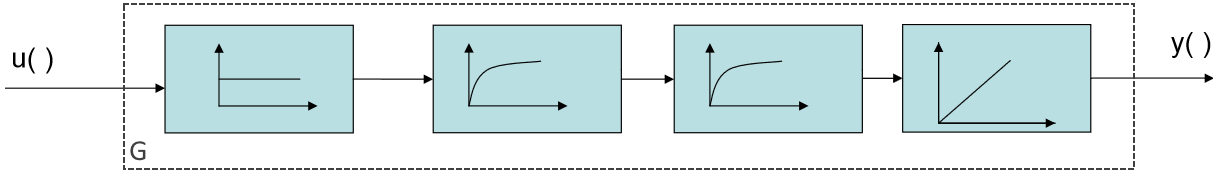
\includegraphics[width=16 cm]{foto/Transmitancja.png}
\caption{Wizualizacja dekompozycji obiektu o transmitancji G }
\label{fig:SCHEMAT}
\end{figure} 

\subsection{Dok�adna transmitancja dyskretna obiektu}
\begin{figure}[H]
\centering
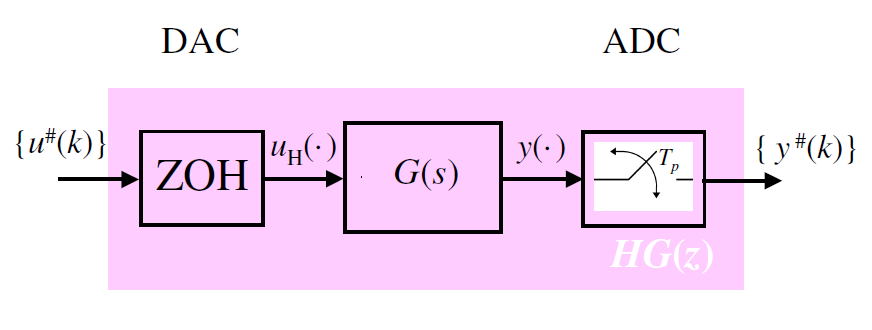
\includegraphics[width=16 cm]{foto/HGz.png}
\caption{Obiekt wraz z uk�adami DAC i ADC}
\label{fig:HGz}
\end{figure} 
Korzystaj�c z wzoru:
\begin{center}
\( HG(z)= \frac{z-1}{z}\mathcal{Z}(\mathcal{L}^{-1} (\frac{G(s)}{s}))= \frac{z-1}{z}\mathcal{D}(\frac{G(s)}{s})\) \\
\end{center}
dla czasu pr�bkowania \(T_p =0.04 \) otrzymano dok�adn� transmitancj� dyskretn� obiektu:
\begin{center}
\( HG(z)= \frac{6.344 \cdot 10^{-6} z^2 +  2.524 \cdot 10^{-5} z + 6.276 \cdot 10^{-6}}{z^3 - 2.979 z^2 + 2.958 z - 0.9788} \) \\
\end{center}

\subsection{Transmitancja widmowa}
Korzystaj�c z zale�no�ci:
\begin{center}
\( HG^*(j\omega )=HG(e^{T_pj\omega}) \)
\end{center}
obliczono transmitancj� widmow�:
\begin{center}
\( HG^*(j\omega )= \frac{6.344 \cdot 10^{-6} (e^{0.041j \omega})^2 +  2.524 \cdot 10^{-5} e^{0.041j \omega} + 6.276 \cdot 10^{-6}}{(e^{0.041j \omega})^3 - 2.979 (e^{0.041j \omega})^2 + 2.958 e^{0.041j \omega} - 0.9788} \)
\end{center}

\subsection{Transmitancja pseudocz�stotliwo�ciowa}
Transmitancja pseudocz�stotliwo�ciowa ma posta�:
\begin{center}
\( HG^{w*}(j\nu)= \frac{1.594 \cdot 10^{-6} j\nu^3 -  8.057 \cdot 10^{-4} j\nu^2 - 1.191 j\nu + 597.9}{j\nu^3 + 5.357 j\nu^2 + 3.986 j\nu}\) \\
\end{center}

Przybli�enie transmitancji pseudocz�stotliwo�ciowej:
\begin{center}
\( HG^{w*}_{est}(j\nu)= G(j\nu)(1-\frac{T_p}{2}j\nu)= \frac{- 0.3 j\nu + 150}{0.2509 j\nu + 1.344 j\nu+ s} \) \\
\end{center}

\begin{figure}[H]
\centering
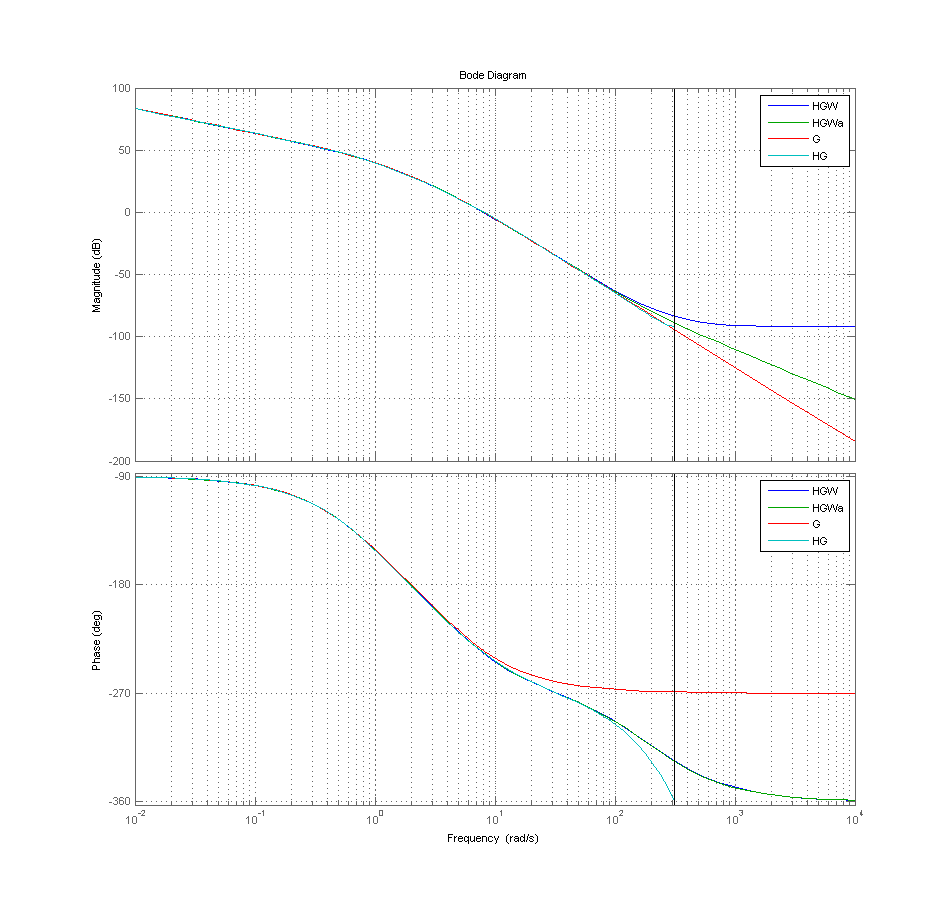
\includegraphics[width=16 cm]{photo/Transfer_functions.png}
\caption{Charakterystyka cz�stotliwo�ciowa transmitancji HGw*, HGw*est, HG* oraz G}
\label{fig:Bode}
\end{figure} 


\section{Projektowanie regulatora}
